\section{From completion to development}
\label{sec:development}

\subsection{Similar completions, different conversion}

A complete color group doubles its base rent. Houses multiply it. The value of a negotiated monopoly therefore depends on what happens at the owner's next management decision, which arrives in the same turn for 35 of the 63 trade-completed groups and within five turns for all but two.

The four systems complete similar numbers of groups by trade: 17 for Sol, 18 for Gemini, 15 for Opus and 13 for Grok. What follows differs sharply (Figure~\ref{fig:conversion}, Table~\ref{tab:conversion}). Sol builds on 16 of its 17 groups in the first management window and Gemini on 17 of 18. Opus builds on 7 of 15 and Grok on 3 of 13. The rent later paid on these groups, until the owner loses them or the game ends, is \$20,818 for Sol and \$26,070 for Gemini against \$5,930 for Opus and \$4,560 for Grok. The 43 groups built on in the first window collect \$53,810 of the \$57,378 total. The 20 others collect \$3,568, although 11 of them are built on later. Construction spending as a whole divides the same way. Sol and Gemini account for \$74,400 of the \$103,450 spent on houses and hotels (Appendix~\ref{app:economy}).

\begin{figure}[t]
\centering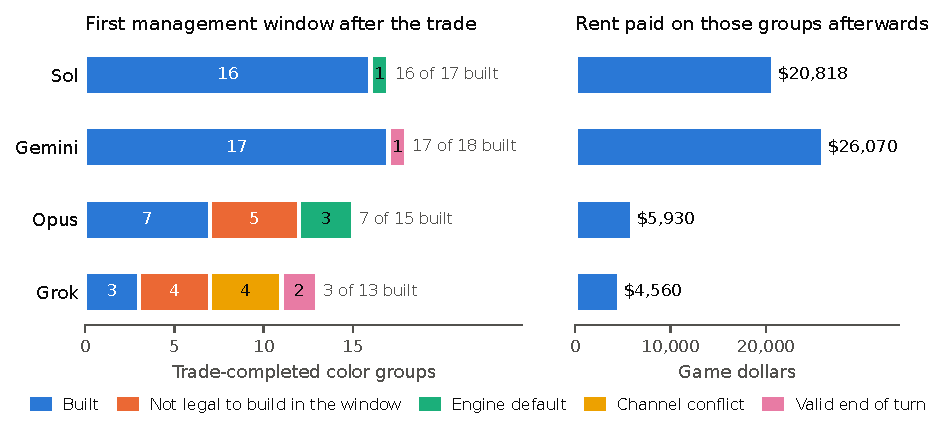
\includegraphics[width=\linewidth]{fig_conversion.pdf}
\caption{The 63 color groups completed by trade, by owner. Left: what happened in the owner's first management window. ``Not legal to build'' means that no decision in the window offered construction on the group. Right: rent paid on the same groups from completion until loss or game end. Windows are not independent, and each row keeps its configuration's response condition (Table~\ref{tab:configurations}).}
\label{fig:conversion}
\end{figure}

\begin{table}[t]
\centering\small
\begin{tabular}{lrrrrrrrr}
\toprule
 & & \multicolumn{2}{c}{Built on} & \multicolumn{4}{c}{First window without building} & \\
\cmidrule(lr){3-4}\cmidrule(lr){5-8}
Owner & Groups & first window & ever & not legal & default & conflict & valid end & Rent\\
\midrule
Sol & 17 & 16 & 17 & 0 & 1 & 0 & 0 & \$20,818\\
Gemini & 18 & 17 & 17 & 0 & 0 & 0 & 1 & \$26,070\\
Opus & 15 & 7 & 12 & 5 & 3 & 0 & 0 & \$5,930\\
Grok & 13 & 3 & 8 & 4 & 0 & 4 & 2 & \$4,560\\
\midrule
All & 63 & 43 & 54 & 9 & 4 & 4 & 3 & \$57,378\\
\bottomrule
\end{tabular}
\caption{Trade-completed groups and their development. ``Default'' is an engine-applied \End{} after failed attempts. ``Conflict'' is a window containing a Grok decision whose text and tool call named different actions. ``Valid end'' is a window of valid selected actions with building legal and none applied. Eighteen of the 63 groups belong to the eventual winner of their game.}
\label{tab:conversion}
\end{table}

The order of these figures matches the order of wins, which invites a causal story the data cannot carry. Rent depends on where rivals land and how long the owner survives, seven wins followed an early monopoly bought from the bank (Section~\ref{sec:setup}), and the two low rows belong to the configurations with nonstandard response conditions. The table does establish where the value of these bargains went, and the reasons are identifiable.

\subsection{Why twenty groups were not built on}

\paragraph{Nine could not legally be built on.} In seven of these the completing deed arrived mortgaged, and the engine forbids building on a group with a mortgaged deed. In the other two the buyer was left with \$158 and \$125 when one house cost \$200. These are properties of the purchase. Four of them are Grok's, all bought from Opus when Opus held under \$70, and Grok's note at each purchase says it will not redeem or build yet. The Boardwalk purchase in Section~\ref{sec:cashpoor} is one. A fifth is Opus's purchase of Park Place in game 15 for \$750 and a utility, the highest price in this group, which left it unable to place a single house.

\paragraph{Four ended in an engine default.} Three are Opus windows in which the first attempt was refused and the action-only retry submitted an invalid build plan. One is a Sol window with two invalid attempts. The engine applied \End{} in each.

\paragraph{Four contain a text and tool-call disagreement.} All are Grok's. In game 20, for example, the first management decision after Grok completes the red group has text describing a mortgage and a tool call that ends the turn (Incident~\ref{inc:boycott}).

\paragraph{Three are valid end-of-turn windows.} Two are Grok's and one is Gemini's. Only in these three was building legal, every action a valid selected response, and nothing built.

Seventeen of the twenty unbuilt windows thus trace to the terms of the acquisition or to the response path. Restricting to the 42 groups that were buildable on entry gives 34 built and eight not, of which three are defaults, three are disagreements and two are valid ends.

\subsection{The default path}
\label{sec:defaults}

Across all management decisions the engine applied a default \End{} 66 times, always after failed construction attempts: 61 for Opus, four for Sol and one for Gemini. Fifty-five of them fall in two games. The failures share a cause. The engine checks the even-building rule after each entry of a build plan, so a plan such as three houses on one deed followed by three on the next is rejected even when the final layout is even.

The earlier audit tested every one of these plans at its exact historical state. All 61 Opus plans execute once each entry is split into single houses and ordered evenly. The cash, the bank stock and the requested purchases are unchanged. Opus asked for affordable, legal allocations in a form the validator rejected, after its one corrective retry had been spent on the provider refusal. Table~\ref{tab:recovery} shows the other systems meeting the same rule with a retry available. They usually end the decision with some construction applied, though Gemini often changes what it buys.

\begin{table}[t]
\centering\small
\begin{tabular}{lrrrr}
\toprule
System & Uneven-plan rejections & Some build applied & Same purchases & Engine default\\
\midrule
Sol & 29 & 25 & 20 & 4\\
Gemini & 19 & 18 & 6 & 1\\
Grok & 5 & 5 & 5 & 0\\
Opus & 61 & 0 & 0 & 61\\
\bottomrule
\end{tabular}
\caption{Decisions in which a build plan was rejected for an uneven intermediate step, followed to resolution. ``Same purchases'' means the applied construction preserved the rejected plan's purchases. In 60 of the 61 Opus decisions the retry had been used by the refusal recovery. Inherited from the earlier audit.}
\label{tab:recovery}
\end{table}

The defaults matter beyond the first window. Of 663 end-of-turn actions applied on menus that offered construction, 66 are these defaults and 24 are Grok decisions whose text named another action. The remaining 573 show no detected conflict, which is not the same as 573 verified decisions to hold cash. An unbuilt monopoly in these games is weak evidence of restraint.

Opus negotiated 15 monopolies and paid for them. It then lost most of their early value to an interaction among a provider refusal, a retry budget and an action format. A count of deals would rate the negotiation as productive and a count of wins would blame the model. The failure sits in the execution layer of the configured system.

\subsection{Liquidity as a target}

Rivals understand that a completed group needs cash, and one incident shows them acting on it.

\IncidentTitle{boycott}{An appeal to withhold a rival's building cash}

In game 20, Opus sells Illinois Avenue to Grok for \$500, which completes Grok's red group on turn 22 and leaves Grok with \$222. A red house costs \$150. Gemini then addresses the table:

\TranscriptQuote{g20-coordination-appeal}

Grok's next private note registers it:

\TranscriptQuote{g20-recognition-note}

Grok's tool call on that decision ends the turn while its text describes a mortgage. At its next decisions it builds three red houses, mortgages New York Avenue and tries to sell a spare deed to Gemini:

\TranscriptQuote{g20-sale-response}

\TranscriptQuote{g20-concrete-refusal}

\IncidentOutcome{Gemini declines the sale and Grok mortgages the deed for \$50. Opus later offers Grok cash for property twice, and neither offer settles. Gemini wins the game.}

\IncidentReading{This is an open attempt to coordinate, named as a boycott by its target, and its author acts on it when given a concrete chance to buy. It is not evidence of a working cartel. Sol had given its own reason for not financing Grok one decision before the appeal, Opus later offered cash anyway, and the record does not show the appeal changing anyone's choice. It does show a system treating a rival's construction budget as a target.}

\IncidentSource{G20 d95--102. Gemini's appeal is in Grok's prompt at d97. The d97 note belongs to the selected second attempt after a malformed first attempt. Grok's red group is one of the four first windows with a text and tool-call disagreement.}
